%%%%%%%%%%%%%%%%%%%%%%%%%%%%%%%%%%%%%%%%%
% Short Sectioned Assignment LaTeX Template Version 1.0 (5/5/12)
% This template has been downloaded from: http://www.LaTeXTemplates.com
% Original author:  Frits Wenneker (http://www.howtotex.com)
% License: CC BY-NC-SA 3.0 (http://creativecommons.org/licenses/by-nc-sa/3.0/)
%%%%%%%%%%%%%%%%%%%%%%%%%%%%%%%%%%%%%%%%%

%----------------------------------------------------------------------------------------
%	PACKAGES AND OTHER DOCUMENT CONFIGURATIONS
%----------------------------------------------------------------------------------------

\documentclass[paper=a4, fontsize=11pt]{scrartcl} % A4 paper and 11pt font size

% ---- Entrada y salida de texto -----

\usepackage[T1]{fontenc} % Use 8-bit encoding that has 256 glyphs
\usepackage[utf8]{inputenc}

% ---- Idioma --------

\usepackage[spanish, es-tabla]{babel} % Selecciona el español para palabras introducidas automáticamente, p.ej. "septiembre" en la fecha y especifica que se use la palabra Tabla en vez de Cuadro

% ---- Otros paquetes ----

\usepackage{amsmath,amsfonts,amsthm} % Math packages
\usepackage{graphics,graphicx, floatrow} %para incluir imágenes y notas en las imágenes
\usepackage{graphics,graphicx, float} %para incluir imágenes y colocarlas
\usepackage{hyperref} % url in references
\usepackage{listings}
\usepackage{color}
\definecolor{grey}{gray}{0.9}

% Para hacer tablas comlejas
\usepackage{multirow}
\usepackage{threeparttable}

\usepackage{fancyhdr} % Custom headers and footers
\pagestyle{fancyplain} % Makes all pages in the document conform to the custom headers and footers
\fancyhead{} % No page header - if you want one, create it in the same way as the footers below
\fancyfoot[L]{} % Empty left footer
\fancyfoot[C]{} % Empty center footer
\fancyfoot[R]{\thepage} % Page numbering for right footer
\renewcommand{\headrulewidth}{0pt} % Remove header underlines
\renewcommand{\footrulewidth}{0pt} % Remove footer underlines
\setlength{\headheight}{13.6pt} % Customize the height of the header

\numberwithin{equation}{section} % Number equations within sections (i.e. 1.1, 1.2, 2.1, 2.2 instead of 1, 2, 3, 4)
\numberwithin{figure}{section} % Number figures within sections (i.e. 1.1, 1.2, 2.1, 2.2 instead of 1, 2, 3, 4)
\numberwithin{table}{section} % Number tables within sections (i.e. 1.1, 1.2, 2.1, 2.2 instead of 1, 2, 3, 4)

\setlength\parindent{0pt} % Removes all indentation from paragraphs - comment this line for an assignment with lots of text

\newcommand{\horrule}[1]{\rule{\linewidth}{#1}} % Create horizontal rule command with 1 argument of height

\usepackage{textcomp}
\usepackage{hyperref}

%----------------------------------------------------------------------------------------
%	DATOS
%----------------------------------------------------------------------------------------

\newcommand{\myName}{Francisco Javier Bolívar Lupiáñez}
\newcommand{\myMail}{fblupi@correo.ugr.es}
\newcommand{\myDNI}{75926571-Y}
\newcommand{\myDegree}{Máster en Ingeniería Informática}
\newcommand{\myFaculty}{E. T. S. de Ingenierías Informática y de Telecomunicación}
\newcommand{\myDepartment}{Ciencias de la Computación e Inteligencia Artificial}
\newcommand{\myUniversity}{\protect{Universidad de Granada}}
\newcommand{\myLocation}{Granada}
\newcommand{\myTime}{\today}
\newcommand{\myTitle}{Práctica 1}
\newcommand{\mySubtitle}{Análisis Preliminar y Visualización Básica de una Red Social de Facebook con Gephi}
\newcommand{\mySubject}{Gestión de Información en la Web}
\newcommand{\myYear}{2016-2017}

%----------------------------------------------------------------------------------------
%	PORTADA
%----------------------------------------------------------------------------------------


\title{	
	\normalfont \normalsize 
	\textsc{\textbf{\mySubject \space (\myYear)} \\ \myDepartment} \\[20pt] % Your university, school and/or department name(s)
	\textsc{\myDegree \\[10pt] \myFaculty \\ \myUniversity} \\[25pt]
	\horrule{0.5pt} \\[0.4cm] % Thin top horizontal rule
	\huge \myTitle: \mySubtitle \\ % The assignment title
	\horrule{2pt} \\[0.5cm] % Thick bottom horizontal rule
	\normalfont \normalsize
}

\author{
	\myName \\
	\small \texttt{\myMail} \\
	\small \myDNI \\
}

\date{\myTime} % Incluye la fecha actual
%----------------------------------------------------------------------------------------
%	INDICE
%----------------------------------------------------------------------------------------

\begin{document}
	
\definecolor{light-gray}{gray}{0.95}
	
\lstset {
	basicstyle=\scriptsize,
	frame=single,
	backgroundcolor=\color{grey}
}
	
\setcounter{page}{0}

\maketitle % Muestra el Título
\thispagestyle{empty}

\newpage %inserta un salto de página

\tableofcontents % para generar el índice de contenidos

\newpage %inserta un salto de página

\listoffigures

\listoftables

\newpage

%----------------------------------------------------------------------------------------
%	DOCUMENTO
%----------------------------------------------------------------------------------------

\section{Introducción}
\label{sec:intro}

En esta práctica se pretende familiarizarse con una herramienta de análisis y visualización de redes sociales como \textit{Gephi}.
\\ \\
Para ello se va a analizar la red de interacciones entre usuarios de un grupo de Facebook extraído con la herramienta \textit{Netvizz}. La cual nos permite descargarnos estos datos siempre y cuando el grupo sea público y tú seas un miembro de éste.
\\ \\
Por lo tanto he escogido el grupo de ``Lobreños por el mundo''. Un grupo que tenemos en mi pueblo de gente que no vive allí pero siempre que puede se escapa para pasar unos días disfrutando de éste. Por tanto, hay gente de distintas partes de Andalucía (Granada, Jaén, Almería o Cádiz), de España (Cataluña o Comunidad Valenciana) e incluso de sudamérica (Brasil o Argentina).

\section{Visualización}

En la Figura \ref{fig:visualizacion} se puede ver la red utilizando el algoritmo ForceAtlas2. La visualización para la componente gigante es igual pues solo hay una componente en la red.

\begin{figure}[H]
	\centering
	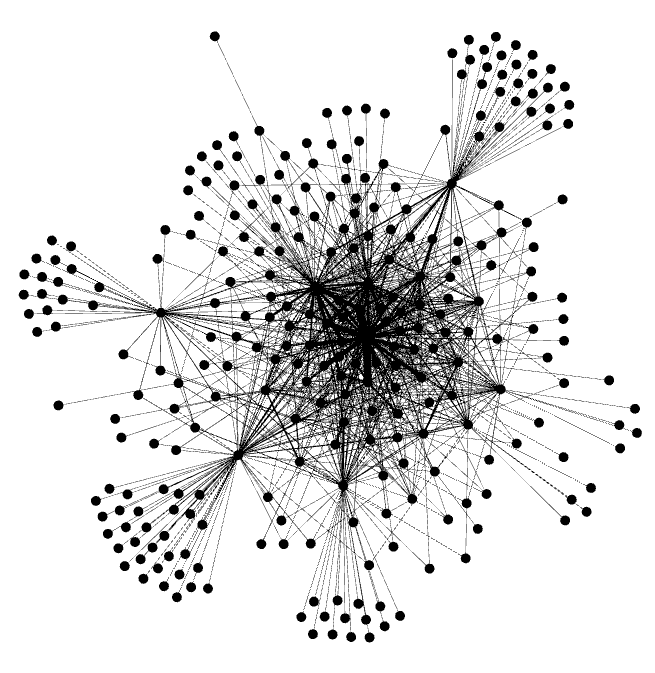
\includegraphics[width=12cm]{img/visualizacion}
	\caption{Visualización usando \textit{ForceAtlas2}}
	\label{fig:visualizacion}
\end{figure}

\section{Valores}

\begin{table}[H]
	\centering
	\caption{Valores de las medidas de análisis de la red original}
	\label{tab:medidas-original}
	\begin{tabular}{| l | l |}
		\hline
		Medida                						& Valor          \\ 
		\hline
		$N$                   						& 284            \\
		$L$                   						& 898            \\
		$L_{max}$                   				& 40186          \\
		$D (\frac{L}{L_{max}})$    					& 0.022          \\
		$k$             							& 6.324          \\
		$d_{max}$									& 5              \\
		$d$                   						& 2.722          \\
		$C$                   						& 0.363          \\
		Componentes conexas   						& 1              \\ 
		$N_{gigante}$         						& 284 (100.0\%)  \\ 
		$L_{gigante}$         						& 898 (100.0\%)  \\ 
		\hline
	\end{tabular}
\end{table}

\begin{figure}[H]
	\centering
	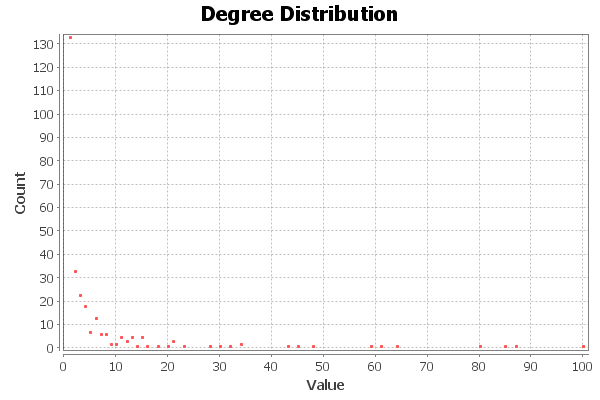
\includegraphics[width=12cm]{img/degree-distribution}
	\caption{Distribución de grados}
	\label{fig:degree-distribution}
\end{figure}

\begin{figure}[H]
	\centering
	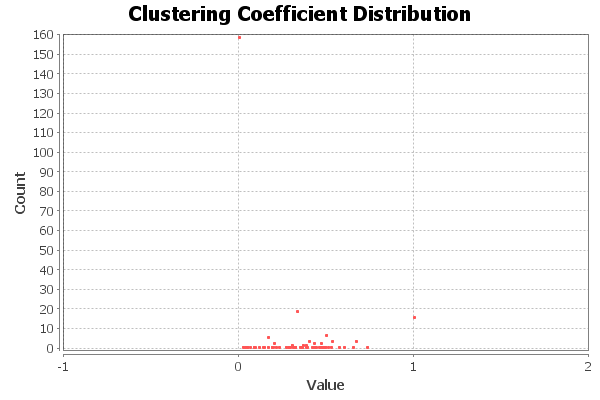
\includegraphics[width=12cm]{img/clustering-coefficient}
	\caption{Distribución de coeficiente de clustering}
	\label{fig:clustering-coefficient}
\end{figure}

\begin{figure}[H]
	\centering
	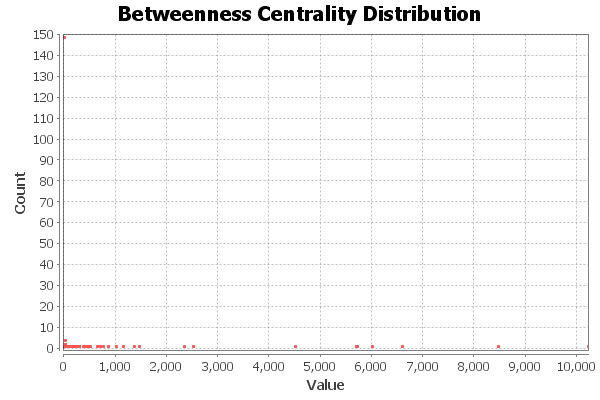
\includegraphics[width=12cm]{img/betweenness-centrality-distribution}
	\caption{Distribución de intermediación}
	\label{fig:betweenness-centrality-distribution}
\end{figure}

\begin{figure}[H]
	\centering
	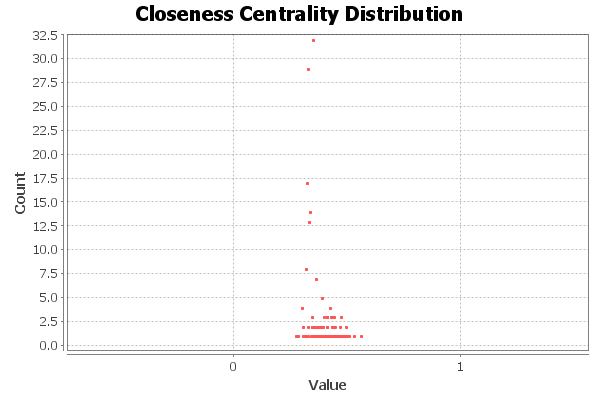
\includegraphics[width=12cm]{img/closeness-centrality-distribution}
	\caption{Distribución de cercanía}
	\label{fig:closeness-centrality-distribution}
\end{figure}

\begin{figure}[H]
	\centering
	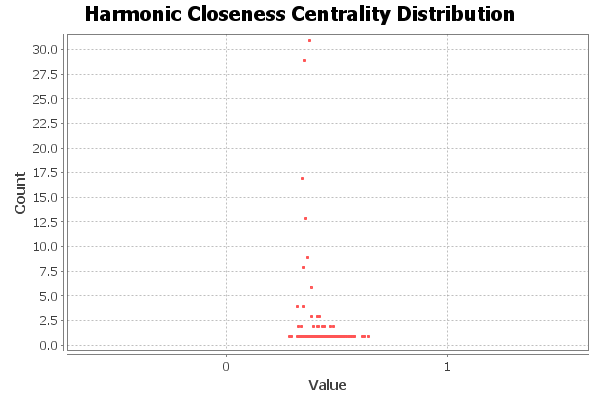
\includegraphics[width=12cm]{img/harmonic-closeness-centrality-distribution}
	\caption{Distribución de cercanía armónica}
	\label{fig:harmonic-closeness-centrality-distribution}
\end{figure}

\begin{figure}[H]
	\centering
	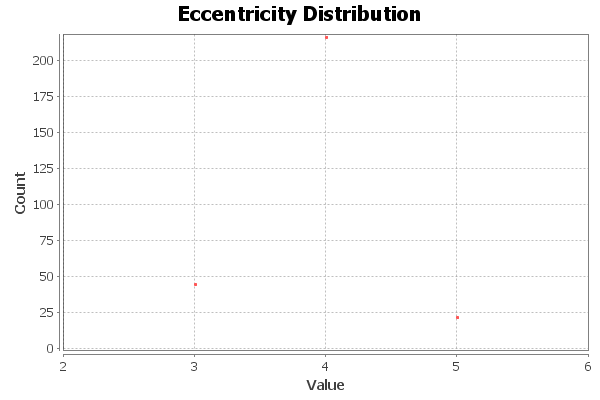
\includegraphics[width=12cm]{img/eccentricity-distribution}
	\caption{Distribución de excentricidad}
	\label{fig:eccentricity-distribution}
\end{figure}

\section{Análisis de la red}

El grado medio es de 6.324 lo que quiere decir que cada nodo interacciona con una media de 6 usuarios. En la Figura \ref{fig:degree-distribution} vemos como sigue la distribución de larga estela. Es decir, la mayoría de los nodos tienen pocos enlaces pero hay unos pocos \textit{hubs} con muchos. Por tanto podríamos decir que es una red libre de escala.
\\ \\
El diámetro es 5 y la distancia media 2.722. Si calculamos la distancia aleatorioa $ \frac{log(N)}{log(log(N))} $ el resultado es 3.417, aún mayor a la distancia media real, por lo que podríamos decir que estamos ante un mundo ultra pequeño.
\\ \\
El coeficiente de clustering es de 0.363 un coeficiente medio-alto que se puede ver en la visualización (Figura \ref{fig:visualizacion}) donde se pueden intuir varios grupos conectados por tan solo un nodo.

%----------------------------------------------------------------------------------------
%	REFERENCIAS
%----------------------------------------------------------------------------------------

\newpage

%\bibliography{referencias} %archivo referencias.bib que contiene las entradas 
%\bibliographystyle{plain} % hay varias formas de citar

\end{document}